\chapter{Teoria dos Jogos}

Neste capítulo, vamos nos concentrar em jogos de dois jogadores que não contêm elementos aleatórios. Nosso objetivo é encontrar uma estratégia que possamos seguir para vencer o jogo, independentemente do que o oponente fizer, se tal estratégia existir.

Veremos que existe uma estratégia geral para tais jogos, e podemos analisá-los usando a \key{teoria nim}. Primeiro, analisaremos jogos simples onde os jogadores removem palitos de pilhas e, depois disso, generalizaremos a estratégia usada nesses jogos para outros jogos.

\section{Estados do Jogo}

Vamos considerar um jogo em que existe inicialmente uma pilha de $n$ palitos. Os jogadores $A$ e $B$ jogam alternadamente, e o jogador $A$ começa. Em cada jogada, o jogador deve remover 1, 2 ou 3 palitos da pilha, e o jogador que remover o último palito vence o jogo.

Por exemplo, se $n=10$, o jogo pode prosseguir da seguinte forma:
\begin{itemize}[noitemsep]
\item Jogador $A$ remove 2 palitos (restam 8 palitos).
\item Jogador $B$ remove 3 palitos (restam 5 palitos).
\item Jogador $A$ remove 1 palito (restam 4 palitos).
\item Jogador $B$ remove 2 palitos (restam 2 palitos).
\item Jogador $A$ remove 2 palitos e vence.
\end{itemize}

Este jogo consiste nos estados $0,1,2,\ldots,n$, onde o número do estado corresponde ao número de palitos restantes.

\subsubsection{Estados de vitória e derrota}

\index{estado de vitória}
\index{estado de derrota}

Um \key{estado de vitória} é um estado em que o jogador vencerá o jogo se jogar de forma otimizada, e um \key{estado de derrota} é um estado em que o jogador perderá o jogo se o oponente jogar de forma otimizada. Podemos classificar todos os estados de um jogo de forma que cada estado seja um estado de vitória ou um estado de derrota.

No jogo acima, o estado 0 é claramente um estado de derrota, porque o jogador não pode fazer nenhuma jogada. Os estados 1, 2 e 3 são estados de vitória, porque podemos remover 1, 2 ou 3 palitos e vencer o jogo. O estado 4, por sua vez, é um estado de derrota, porque qualquer jogada leva a um estado que é um estado de vitória para o oponente.

De forma mais geral, se houver uma jogada que leva do estado atual para um estado de derrota, o estado atual é um estado de vitória; caso contrário, o estado atual é um estado de derrota. Usando essa observação, podemos classificar todos os estados de um jogo, começando com os estados de derrota onde não há jogadas possíveis.

Os estados $0 \ldots 15$ do jogo acima podem ser classificados da seguinte forma ($V$ denota um estado de vitória e $D$ denota um estado de derrota):

\begin{center}
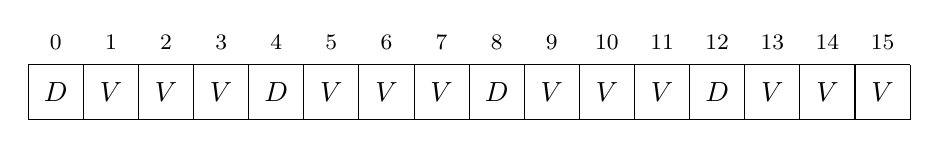
\begin{tikzpicture}[scale=0.7]
\draw (0,0) grid (16,1);

\node at (0.5,0.5) {$D$};
\node at (1.5,0.5) {$V$};
\node at (2.5,0.5) {$V$};
\node at (3.5,0.5) {$V$};
\node at (4.5,0.5) {$D$};
\node at (5.5,0.5) {$V$};
\node at (6.5,0.5) {$V$};
\node at (7.5,0.5) {$V$};
\node at (8.5,0.5) {$D$};
\node at (9.5,0.5) {$V$};
\node at (10.5,0.5) {$V$};
\node at (11.5,0.5) {$V$};
\node at (12.5,0.5) {$D$};
\node at (13.5,0.5) {$V$};
\node at (14.5,0.5) {$V$};
\node at (15.5,0.5) {$V$};

\footnotesize
\node at (0.5,1.4) {$0$};
\node at (1.5,1.4) {$1$};
\node at (2.5,1.4) {$2$};
\node at (3.5,1.4) {$3$};
\node at (4.5,1.4) {$4$};
\node at (5.5,1.4) {$5$};
\node at (6.5,1.4) {$6$};
\node at (7.5,1.4) {$7$};
\node at (8.5,1.4) {$8$};
\node at (9.5,1.4) {$9$};
\node at (10.5,1.4) {$10$};
\node at (11.5,1.4) {$11$};
\node at (12.5,1.4) {$12$};
\node at (13.5,1.4) {$13$};
\node at (14.5,1.4) {$14$};
\node at (15.5,1.4) {$15$};
\end{tikzpicture}
\end{center}

É fácil analisar este jogo: um estado $k$ é um estado de derrota se $k$ for divisível por 4 e, caso contrário, é um estado de vitória. Uma maneira ideal de jogar é sempre escolher uma jogada após a qual o número de palitos na pilha seja divisível por 4. Finalmente, não haverá mais palitos e o oponente terá perdido.

Claro, esta estratégia exige que o número de palitos \emph{não} seja divisível por 4 quando for a nossa vez. Se for, não há nada que possamos fazer, e o oponente vencerá o jogo se jogar de forma otimizada.

\subsubsection{Grafo de estados}

Vamos agora considerar outro jogo de palitos, onde em cada estado $k$, é permitido remover qualquer número $x$ de palitos tal que $x$ seja menor que $k$ e divida $k$. Por exemplo, no estado 8 podemos remover 1, 2 ou 4 palitos, mas no estado 7 a única jogada permitida é remover 1 palito.

A figura a seguir mostra os estados $1 \ldots 9$ do jogo como um \key{grafo de estados}, cujos nós são os estados e as arestas são as jogadas entre eles:

\begin{center}
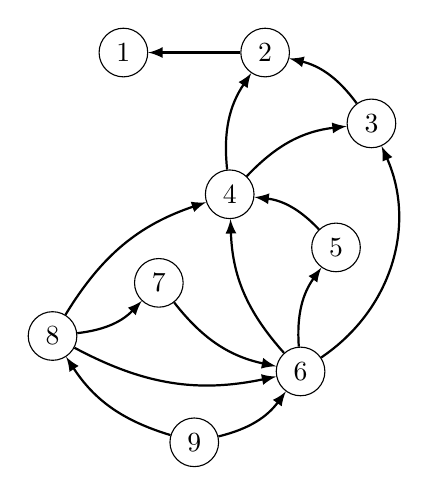
\begin{tikzpicture}[scale=0.9]
\node[draw, circle] (1) at (0,0) {$1$};
\node[draw, circle] (2) at (2,0) {$2$};
\node[draw, circle] (3) at (3.5,-1) {$3$};
\node[draw, circle] (4) at (1.5,-2) {$4$};
\node[draw, circle] (5) at (3,-2.75) {$5$};
\node[draw, circle] (6) at (2.5,-4.5) {$6$};
\node[draw, circle] (7) at (0.5,-3.25) {$7$};
\node[draw, circle] (8) at (-1,-4) {$8$};
\node[draw, circle] (9) at (1,-5.5) {$9$};

\path[draw,thick,->,>=latex] (2) -- (1);
\path[draw,thick,->,>=latex] (3) edge [bend right=20] (2);
\path[draw,thick,->,>=latex] (4) edge [bend left=20] (2);
\path[draw,thick,->,>=latex] (4) edge [bend left=20] (3);
\path[draw,thick,->,>=latex] (5) edge [bend right=20] (4);
\path[draw,thick,->,>=latex] (6) edge [bend left=20] (5);
\path[draw,thick,->,>=latex] (6) edge [bend left=20] (4);
\path[draw,thick,->,>=latex] (6) edge [bend right=40] (3);
\path[draw,thick,->,>=latex] (7) edge [bend right=20] (6);
\path[draw,thick,->,>=latex] (8) edge [bend right=20] (7);
\path[draw,thick,->,>=latex] (8) edge [bend right=20] (6);
\path[draw,thick,->,>=latex] (8) edge [bend left=20] (4);
\path[draw,thick,->,>=latex] (9) edge [bend left=20] (8);
\path[draw,thick,->,>=latex] (9) edge [bend right=20] (6);
\end{tikzpicture}
\end{center}

O estado final neste jogo é sempre o estado 1, que é um estado de derrota, porque não há jogadas válidas. A classificação dos estados $1 \ldots 9$ é a seguinte:

\begin{center}
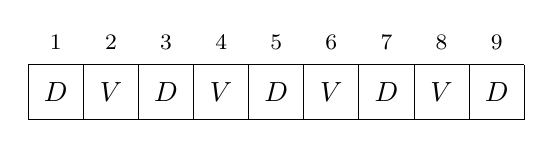
\begin{tikzpicture}[scale=0.7]
\draw (1,0) grid (10,1);

\node at (1.5,0.5) {$D$};
\node at (2.5,0.5) {$V$};
\node at (3.5,0.5) {$D$};
\node at (4.5,0.5) {$V$};
\node at (5.5,0.5) {$D$};
\node at (6.5,0.5) {$V$};
\node at (7.5,0.5) {$D$};
\node at (8.5,0.5) {$V$};
\node at (9.5,0.5) {$D$};

\footnotesize
\node at (1.5,1.4) {$1$};
\node at (2.5,1.4) {$2$};
\node at (3.5,1.4) {$3$};
\node at (4.5,1.4) {$4$};
\node at (5.5,1.4) {$5$};
\node at (6.5,1.4) {$6$};
\node at (7.5,1.4) {$7$};
\node at (8.5,1.4) {$8$};
\node at (9.5,1.4) {$9$};
\end{tikzpicture}
\end{center}

Surpreendentemente, neste jogo, todos os estados pares são estados de vitória e todos os estados ímpares são estados de derrota.

\section{Jogo Nim}

\index{jogo nim}

O \key{jogo nim} é um jogo simples que tem um papel importante na teoria dos jogos, porque muitos outros jogos podem ser jogados usando a mesma estratégia. Primeiro, vamos nos concentrar no nim e, em seguida, generalizaremos a estratégia para outros jogos.

Existem $n$ pilhas no nim, e cada pilha contém um certo número de palitos. Os jogadores jogam alternadamente e, em cada turno, o jogador escolhe uma pilha que ainda contém palitos e remove qualquer número de palitos dela. O vencedor é o jogador que remover o último palito.

Os estados no nim são da forma $[x_1,x_2,\ldots,x_n]$, onde $x_k$ denota o número de palitos na pilha $k$. Por exemplo, $[10,12,5]$ é um jogo onde existem três pilhas com 10, 12 e 5 palitos. O estado $[0,0,\ldots,0]$ é um estado de derrota, porque não é possível remover nenhum palito, e este é sempre o estado final.

\subsubsection{Análise}
\index{soma nim}

Acontece que podemos classificar facilmente qualquer estado nim calculando a \key{soma nim} $s = x_1 \oplus x_2 \oplus \cdots \oplus x_n$, onde $\oplus$ é a operação xor\footnote{A estratégia ideal para nim foi publicada em 1901 por C. L. Bouton \cite{bou01}.}. Os estados cuja soma nim é 0 são estados de derrota e todos os outros estados são estados de vitória. Por exemplo, a soma nim de $[10,12,5]$ é $10 \oplus 12 \oplus 5 = 3$, então o estado é um estado de vitória.

Mas como a soma nim está relacionada ao jogo nim? Podemos explicar isso observando como a soma nim muda quando o estado nim muda.

\textit{Estados de derrota:} O estado final $[0,0,\ldots,0]$ é um estado de derrota e sua soma nim é 0, como esperado. Em outros estados de derrota, qualquer jogada leva a um estado de vitória, porque quando um único valor $x_k$ muda, a soma nim também muda, então a soma nim é diferente de 0 após a jogada.

\textit{Estados de vitória:} Podemos ir para um estado de derrota se houver alguma pilha $k$ para a qual $x_k \oplus s < x_k$. Nesse caso, podemos remover palitos da pilha $k$ para que ela contenha $x_k \oplus s$ palitos, o que levará a um estado de derrota. Sempre existe tal pilha, onde $x_k$ tem um bit 1 na posição do bit 1 mais à esquerda de $s$.

Como exemplo, considere o estado $[10,12,5]$. Este estado é um estado de vitória, porque sua soma nim é 3. Portanto, deve haver uma jogada que leva a um estado de derrota. A seguir, descobriremos tal jogada.

A soma nim do estado é a seguinte:

\begin{center}
\begin{tabular}{r|r}
10 & \texttt{1010} \\
12 & \texttt{1100} \\
5 & \texttt{0101} \\
\hline
3 & \texttt{0011} \\
\end{tabular}
\end{center}

Neste caso, a pilha com 10 palitos é a única pilha que possui um bit 1 na posição do bit 1 mais à esquerda da soma nim:

\begin{center}
\begin{tabular}{r|r}
10 & \texttt{10\underline{1}0} \\
12 & \texttt{1100} \\
5 & \texttt{0101} \\
\hline
3 & \texttt{00\underline{1}1} \\
\end{tabular}
\end{center}

O novo tamanho da pilha deve ser $10 \oplus 3 = 9$, então removeremos apenas um palito. Depois disso, o estado será $[9,12,5]$, que é um estado de derrota:

\begin{center}
\begin{tabular}{r|r}
9 & \texttt{1001} \\
12 & \texttt{1100} \\
5 & \texttt{0101} \\
\hline
0 & \texttt{0000} \\
\end{tabular}
\end{center}

\subsubsection{Jogo Misère}

\index{jogo misère}

Em um \key{jogo misère}, o objetivo do jogo é oposto, então o jogador que remove o último palito perde o jogo. Acontece que o jogo nim misère pode ser jogado de forma ideal quase como o jogo nim padrão.

A ideia é primeiro jogar o jogo misère como o jogo padrão, mas mudar a estratégia no final do jogo. A nova estratégia será introduzida em uma situação em que cada pilha conteria no máximo um palito após a próxima jogada.

No jogo padrão, devemos escolher uma jogada após a qual haja um número par de pilhas com um palito. No entanto, no jogo misère, escolhemos uma jogada de forma que haja um número ímpar de pilhas com um palito.

Essa estratégia funciona porque um estado onde a estratégia muda sempre aparece no jogo, e esse estado é um estado de vitória, porque contém exatamente uma pilha que possui mais de um palito, então a soma nim não é 0.

\section{Teorema de Sprague–Grundy}

\index{Teorema de Sprague–Grundy}

O \key{Teorema de Sprague–Grundy}\footnote{O teorema foi descoberto independentemente por R. Sprague \cite{spr35} e P. M. Grundy \cite{gru39}.} generaliza a estratégia usada no nim para todos os jogos que atendem aos seguintes requisitos:

\begin{itemize}[noitemsep]
\item Existem dois jogadores que jogam alternadamente.
\item O jogo consiste em estados, e as jogadas possíveis em um estado não dependem de quem é a vez.
\item O jogo termina quando um jogador não pode mais fazer uma jogada.
\item O jogo certamente termina mais cedo ou mais tarde.
\item Os jogadores têm informações completas sobre os estados e as jogadas permitidas, e não há aleatoriedade no jogo.
\end{itemize}

A ideia é calcular, para cada estado do jogo, um número de Grundy que corresponde ao número de palitos em uma pilha nim. Quando sabemos os números de Grundy de todos os estados, podemos jogar como o jogo nim.

\subsubsection{Números de Grundy}

\index{Número de Grundy}
\index{função mex}

O \key{Número de Grundy} de um estado do jogo é
\[\textrm{mex}(\{g_1,g_2,\ldots,g_n\}),\]
onde $g_1,g_2,\ldots,g_n$ são os números de Grundy dos estados para os quais podemos mover, e a função mex retorna o menor número inteiro não negativo que não está no conjunto. Por exemplo, $\textrm{mex}(\{0,1,3\})=2$. Se não houver jogadas possíveis em um estado, seu número de Grundy é 0, porque $\textrm{mex}(\emptyset)=0$.

Por exemplo, no grafo de estados:
\begin{center}
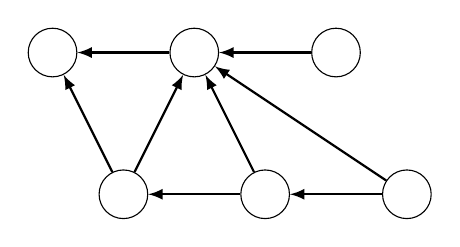
\begin{tikzpicture}[scale=0.9]
\node[draw, circle] (1) at (0,0) {\phantom{0}};
\node[draw, circle] (2) at (2,0) {\phantom{0}};
\node[draw, circle] (3) at (4,0) {\phantom{0}};
\node[draw, circle] (4) at (1,-2) {\phantom{0}};
\node[draw, circle] (5) at (3,-2) {\phantom{0}};
\node[draw, circle] (6) at (5,-2) {\phantom{0}};

\path[draw,thick,->,>=latex] (2) -- (1);
\path[draw,thick,->,>=latex] (3) -- (2);
\path[draw,thick,->,>=latex] (5) -- (4);
\path[draw,thick,->,>=latex] (6) -- (5);
\path[draw,thick,->,>=latex] (4) -- (1);
\path[draw,thick,->,>=latex] (4) -- (2);
\path[draw,thick,->,>=latex] (5) -- (2);
\path[draw,thick,->,>=latex] (6) -- (2);
\end{tikzpicture}
\end{center}

os números de Grundy são os seguintes:
\begin{center}
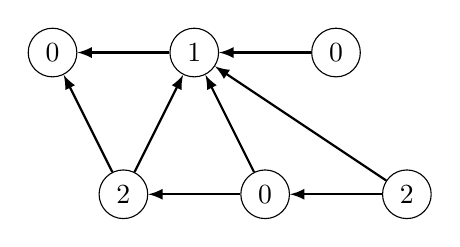
\begin{tikzpicture}[scale=0.9]
\node[draw, circle] (1) at (0,0) {0};
\node[draw, circle] (2) at (2,0) {1};
\node[draw, circle] (3) at (4,0) {0};
\node[draw, circle] (4) at (1,-2) {2};
\node[draw, circle] (5) at (3,-2) {0};
\node[draw, circle] (6) at (5,-2) {2};

\path[draw,thick,->,>=latex] (2) -- (1);
\path[draw,thick,->,>=latex] (3) -- (2);
\path[draw,thick,->,>=latex] (5) -- (4);
\path[draw,thick,->,>=latex] (6) -- (5);
\path[draw,thick,->,>=latex] (4) -- (1);
\path[draw,thick,->,>=latex] (4) -- (2);
\path[draw,thick,->,>=latex] (5) -- (2);
\path[draw,thick,->,>=latex] (6) -- (2);
\end{tikzpicture}
\end{center}

O número de Grundy de um estado de derrota é 0, e o número de Grundy de um estado de vitória é um número positivo.

O número de Grundy de um estado corresponde ao número de palitos em uma pilha nim. Se o número de Grundy for 0, podemos mover apenas para estados cujos números de Grundy são positivos, e se o número de Grundy for $x>0$, podemos mover para estados cujos números de Grundy incluem todos os números $0,1,\ldots,x-1$.

Como exemplo, considere um jogo onde os jogadores movem uma peça em um labirinto. Cada quadrado no labirinto é um chão ou uma parede. A cada turno, o jogador deve mover a peça um certo número de passos para a esquerda ou para cima. O vencedor do jogo é o jogador que fizer o último movimento.

A figura a seguir mostra um possível estado inicial do jogo, onde @ denota a peça e * denota um quadrado para onde ela pode se mover.

\begin{center}
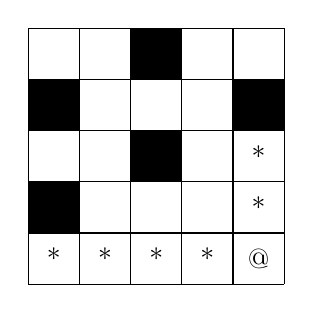
\begin{tikzpicture}[scale=.65]
  \begin{scope}
    \fill [color=black] (0, 1) rectangle (1, 2);
    \fill [color=black] (0, 3) rectangle (1, 4);
    \fill [color=black] (2, 2) rectangle (3, 3);
    \fill [color=black] (2, 4) rectangle (3, 5);
    \fill [color=black] (4, 3) rectangle (5, 4);

    \draw (0, 0) grid (5, 5);
    
    \node at (4.5,0.5) {@};
    \node at (3.5,0.5) {*};
    \node at (2.5,0.5) {*};
    \node at (1.5,0.5) {*};
    \node at (0.5,0.5) {*};
    \node at (4.5,1.5) {*};
    \node at (4.5,2.5) {*};
    
  \end{scope}
\end{tikzpicture}
\end{center}

Os estados do jogo são todos os quadrados do chão do labirinto. No labirinto acima, os números de Grundy são os seguintes:

\begin{center}
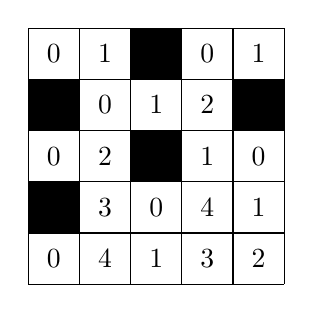
\begin{tikzpicture}[scale=.65]
  \begin{scope}
    \fill [color=black] (0, 1) rectangle (1, 2);
    \fill [color=black] (0, 3) rectangle (1, 4);
    \fill [color=black] (2, 2) rectangle (3, 3);
    \fill [color=black] (2, 4) rectangle (3, 5);
    \fill [color=black] (4, 3) rectangle (5, 4);

    \draw (0, 0) grid (5, 5);
    
    \node at (0.5,4.5) {0};
    \node at (1.5,4.5) {1};
    \node at (2.5,4.5) {};
    \node at (3.5,4.5) {0};
    \node at (4.5,4.5) {1};

    \node at (0.5,3.5) {};
    \node at (1.5,3.5) {0};
    \node at (2.5,3.5) {1};
    \node at (3.5,3.5) {2};
    \node at (4.5,3.5) {};

    \node at (0.5,2.5) {0};
    \node at (1.5,2.5) {2};
    \node at (2.5,2.5) {};
    \node at (3.5,2.5) {1};
    \node at (4.5,2.5) {0};

    \node at (0.5,1.5) {};
    \node at (1.5,1.5) {3};
    \node at (2.5,1.5) {0};
    \node at (3.5,1.5) {4};
    \node at (4.5,1.5) {1};

    \node at (0.5,0.5) {0};
    \node at (1.5,0.5) {4};
    \node at (2.5,0.5) {1};
    \node at (3.5,0.5) {3};
    \node at (4.5,0.5) {2};
  \end{scope}
\end{tikzpicture}
\end{center}

Assim, cada estado do jogo do labirinto corresponde a uma pilha no jogo nim. Por exemplo, o número de Grundy para o quadrado inferior direito é 2, então é um estado de vitória. Podemos chegar a um estado de derrota e vencer o jogo movendo quatro passos para a esquerda ou dois passos para cima.

Observe que, ao contrário do jogo nim original, pode ser possível mover para um estado cujo número de Grundy seja maior do que o número de Grundy do estado atual. No entanto, o oponente sempre pode escolher uma jogada que cancele tal movimento, então não é possível escapar de um estado de derrota.

\subsubsection{Subjogos}

A seguir, assumiremos que nosso jogo consiste em subjogos e, em cada turno, o jogador primeiro escolhe um subjogo e, em seguida, uma jogada no subjogo. O jogo termina quando não é possível fazer nenhuma jogada em nenhum subjogo.

Neste caso, o número de Grundy de um jogo é a soma nim dos números de Grundy dos subjogos. O jogo pode ser jogado como um jogo nim calculando todos os números de Grundy para subjogos e, em seguida, sua soma nim.

Como exemplo, considere um jogo que consiste em três labirintos. Neste jogo, em cada turno, o jogador escolhe um dos labirintos e então move a peça no labirinto. Suponha que o estado inicial do jogo seja o seguinte:

\begin{center}
\begin{tabular}{ccc}
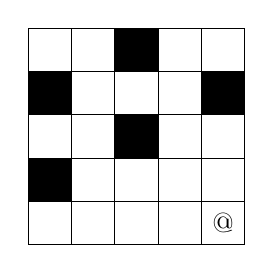
\begin{tikzpicture}[scale=.55]
  \begin{scope}
    \fill [color=black] (0, 1) rectangle (1, 2);
    \fill [color=black] (0, 3) rectangle (1, 4);
    \fill [color=black] (2, 2) rectangle (3, 3);
    \fill [color=black] (2, 4) rectangle (3, 5);
    \fill [color=black] (4, 3) rectangle (5, 4);

    \draw (0, 0) grid (5, 5);

    \node at (4.5,0.5) {@};

    \end{scope}
\end{tikzpicture}
&
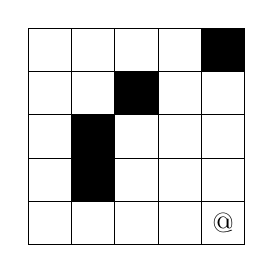
\begin{tikzpicture}[scale=.55]
  \begin{scope}
    \fill [color=black] (1, 1) rectangle (2, 3);
    \fill [color=black] (2, 3) rectangle (3, 4);
    \fill [color=black] (4, 4) rectangle (5, 5);

    \draw (0, 0) grid (5, 5);
    
    \node at (4.5,0.5) {@};

  \end{scope}
\end{tikzpicture}
&
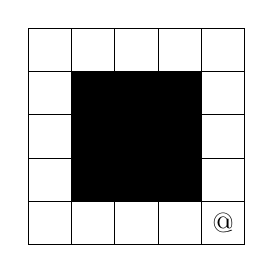
\begin{tikzpicture}[scale=.55]
  \begin{scope}
    \fill [color=black] (1, 1) rectangle (4, 4);

    \draw (0, 0) grid (5, 5);
    
    \node at (4.5,0.5) {@};
  \end{scope}
\end{tikzpicture}
\end{tabular}
\end{center}

Os números de Grundy para os labirintos são os seguintes:

\begin{center}
\begin{tabular}{ccc}
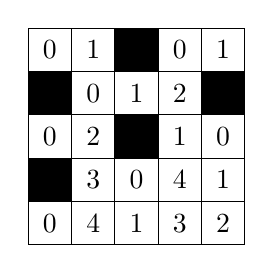
\begin{tikzpicture}[scale=.55]
  \begin{scope}
    \fill [color=black] (0, 1) rectangle (1, 2);
    \fill [color=black] (0, 3) rectangle (1, 4);
    \fill [color=black] (2, 2) rectangle (3, 3);
    \fill [color=black] (2, 4) rectangle (3, 5);
    \fill [color=black] (4, 3) rectangle (5, 4);

    \draw (0, 0) grid (5, 5);

    \node at (0.5,4.5) {0};
    \node at (1.5,4.5) {1};
    \node at (2.5,4.5) {};
    \node at (3.5,4.5) {0};
    \node at (4.5,4.5) {1};

    \node at (0.5,3.5) {};
    \node at (1.5,3.5) {0};
    \node at (2.5,3.5) {1};
    \node at (3.5,3.5) {2};
    \node at (4.5,3.5) {};

    \node at (0.5,2.5) {0};
    \node at (1.5,2.5) {2};
    \node at (2.5,2.5) {};
    \node at (3.5,2.5) {1};
    \node at (4.5,2.5) {0};

    \node at (0.5,1.5) {};
    \node at (1.5,1.5) {3};
    \node at (2.5,1.5) {0};
    \node at (3.5,1.5) {4};
    \node at (4.5,1.5) {1};

    \node at (0.5,0.5) {0};
    \node at (1.5,0.5) {4};
    \node at (2.5,0.5) {1};
    \node at (3.5,0.5) {3};
    \node at (4.5,0.5) {2};
    \end{scope}
\end{tikzpicture}
&
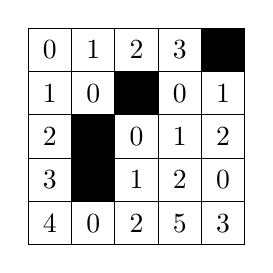
\begin{tikzpicture}[scale=.55]
  \begin{scope}
    \fill [color=black] (1, 1) rectangle (2, 3);
    \fill [color=black] (2, 3) rectangle (3, 4);
    \fill [color=black] (4, 4) rectangle (5, 5);

    \draw (0, 0) grid (5, 5);

    \node at (0.5,4.5) {0};
    \node at (1.5,4.5) {1};
    \node at (2.5,4.5) {2};
    \node at (3.5,4.5) {3};
    \node at (4.5,4.5) {};

    \node at (0.5,3.5) {1};
    \node at (1.5,3.5) {0};
    \node at (2.5,3.5) {};
    \node at (3.5,3.5) {0};
    \node at (4.5,3.5) {1};

    \node at (0.5,2.5) {2};
    \node at (1.5,2.5) {};
    \node at (2.5,2.5) {0};
    \node at (3.5,2.5) {1};
    \node at (4.5,2.5) {2};

    \node at (0.5,1.5) {3};
    \node at (1.5,1.5) {};
    \node at (2.5,1.5) {1};
    \node at (3.5,1.5) {2};
    \node at (4.5,1.5) {0};

    \node at (0.5,0.5) {4};
    \node at (1.5,0.5) {0};
    \node at (2.5,0.5) {2};
    \node at (3.5,0.5) {5};
    \node at (4.5,0.5) {3};
  \end{scope}
\end{tikzpicture}
&
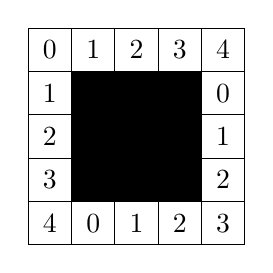
\begin{tikzpicture}[scale=.55]
  \begin{scope}
    \fill [color=black] (1, 1) rectangle (4, 4);

    \draw (0, 0) grid (5, 5);

    \node at (0.5,4.5) {0};
    \node at (1.5,4.5) {1};
    \node at (2.5,4.5) {2};
    \node at (3.5,4.5) {3};
    \node at (4.5,4.5) {4};

    \node at (0.5,3.5) {1};
    \node at (1.5,3.5) {};
    \node at (2.5,3.5) {};
    \node at (3.5,3.5) {};
    \node at (4.5,3.5) {0};

    \node at (0.5,2.5) {2};
    \node at (1.5,2.5) {};
    \node at (2.5,2.5) {};
    \node at (3.5,2.5) {};
    \node at (4.5,2.5) {1};

    \node at (0.5,1.5) {3};
    \node at (1.5,1.5) {};
    \node at (2.5,1.5) {};
    \node at (3.5,1.5) {};
    \node at (4.5,1.5) {2};

    \node at (0.5,0.5) {4};
    \node at (1.5,0.5) {0};
    \node at (2.5,0.5) {1};
    \node at (3.5,0.5) {2};
    \node at (4.5,0.5) {3};
  \end{scope}
\end{tikzpicture}
\end{tabular}
\end{center}

No estado inicial, a soma nim dos números de Grundy é $2 \oplus 3 \oplus 3 = 2$, então o primeiro jogador pode vencer o jogo. Uma jogada ideal é mover dois passos para cima no primeiro labirinto, o que produz a soma nim $0 \oplus 3 \oplus 3 = 0$.

\subsubsection{Jogo de Grundy}

Às vezes, uma jogada em um jogo divide o jogo em subjogos independentes um do outro. Neste caso, o número de Grundy do jogo é
\[\textrm{mex}(\{g_1, g_2, \ldots, g_n \}),\]
onde $n$ é o número de jogadas possíveis e
\[g_k = a_{k,1} \oplus a_{k,2} \oplus \ldots \oplus a_{k,m},\]
onde a jogada $k$ gera subjogos com números de Grundy $a_{k,1},a_{k,2},\ldots,a_{k,m}$.

\index{Jogo de Grundy}

Um exemplo de tal jogo é o \key{Jogo de Grundy}. Inicialmente, existe uma única pilha que contém $n$ palitos. Em cada turno, o jogador escolhe uma pilha e a divide em duas pilhas não vazias, de modo que as pilhas tenham tamanhos diferentes. O jogador que fizer o último movimento vence o jogo.

Seja $f(n)$ o número de Grundy de uma pilha que contém $n$ palitos. O número de Grundy pode ser calculado percorrendo todas as maneiras de dividir a pilha em duas pilhas. Por exemplo, quando $n=8$, as possibilidades são $1+7$, $2+6$ e $3+5$, então
\[f(8)=\textrm{mex}(\{f(1) \oplus f(7), f(2) \oplus f(6), f(3) \oplus f(5)\}).\]

Neste jogo, o valor de $f(n)$ é baseado nos valores de $f(1),\ldots,f(n-1)$. Os casos base são $f(1)=f(2)=0$, porque não é possível dividir as pilhas de 1 e 2 palitos. Os primeiros números de Grundy são:

\[
\begin{array}{lcl}
f(1) & = & 0 \\
f(2) & = & 0 \\
f(3) & = & 1 \\
f(4) & = & 0 \\
f(5) & = & 2 \\
f(6) & = & 1 \\
f(7) & = & 0 \\
f(8) & = & 2 \\
\end{array}
\]

O número de Grundy para $n=8$ é 2, então é possível vencer o jogo. A jogada vencedora é criar pilhas $1+7$, porque $f(1) \oplus f(7) = 0$.
